%%%%%%%%%%%%%%%%%%%%%%%%%%%%%%%%%%%%%%%%%
% Arsclassica Article
% LaTeX Template
% Version 1.1 (1/8/17)
%
% This template has been downloaded from:
% http://www.LaTeXTemplates.com
%
% Original author:
% Lorenzo Pantieri (http://www.lorenzopantieri.net) with extensive modifications by:
% Vel (vel@latextemplates.com)
%
% License:
% CC BY-NC-SA 3.0 (http://creativecommons.org/licenses/by-nc-sa/3.0/)
%
%%%%%%%%%%%%%%%%%%%%%%%%%%%%%%%%%%%%%%%%%

%----------------------------------------------------------------------------------------
%	PACKAGES AND OTHER DOCUMENT CONFIGURATIONS
%----------------------------------------------------------------------------------------
\documentclass[
11pt, % Main document font size
a4paper, % Paper type, use 'letterpaper' for US Letter paper
oneside, % One page layout (no page indentation)
%twoside, % Two page layout (page indentation for binding and different headers)
headinclude,footinclude, % Extra spacing for the header and footer
BCOR5mm, % Binding correction
]{scrartcl}

% configuration file where all the packages are loaded and set up
% commands new/redefined are done in here
%%%%%%%%%%%%%%%%%%%%%%%%%%%%%%%%%%%%%%%%%
% Arsclassica Article
% Structure Specification File
%
% This file has been downloaded from:
% http://www.LaTeXTemplates.com
%
% Original author:
% Lorenzo Pantieri (http://www.lorenzopantieri.net) with extensive modifications by:
% Vel (vel@latextemplates.com)
%
% License:
% CC BY-NC-SA 3.0 (http://creativecommons.org/licenses/by-nc-sa/3.0/)
%
%%%%%%%%%%%%%%%%%%%%%%%%%%%%%%%%%%%%%%%%%

%----------------------------------------------------------------------------------------
%	REQUIRED PACKAGES
%----------------------------------------------------------------------------------------

\usepackage[
nochapters, % Turn off chapters since this is an article        
beramono, % Use the Bera Mono font for monospaced text (\texttt)
eulermath,% Use the Euler font for mathematics
pdfspacing, % Makes use of pdftex’ letter spacing capabilities via the microtype package
dottedtoc % Dotted lines leading to the page numbers in the table of contents
]{classicthesis} % The layout is based on the Classic Thesis style

\usepackage{url} % Allows usage of hyperlinks
\usepackage{arsclassica} % Modifies the Classic Thesis package
\usepackage[T1]{fontenc} % Use 8-bit encoding that has 256 glyphs
\usepackage[utf8]{inputenc} % Required for including letters with accents
\usepackage[swedish, english]{babel}
\usepackage{graphicx} % Required for including images
\usepackage{enumitem} % Required for manipulating the whitespace between and within lists
\usepackage{lipsum} % Used for inserting dummy 'Lorem ipsum' text into the template
\usepackage{subfig} % Required for creating figures with multiple parts (subfigures)
\usepackage{amsmath,amssymb,amsthm} % For including math equations, theorems, symbols, etc
\usepackage{varioref} % More descriptive referencing

\usepackage[pages=some, scale=1, angle=0, opacity=0.7]{background}
\backgroundsetup{
  contents={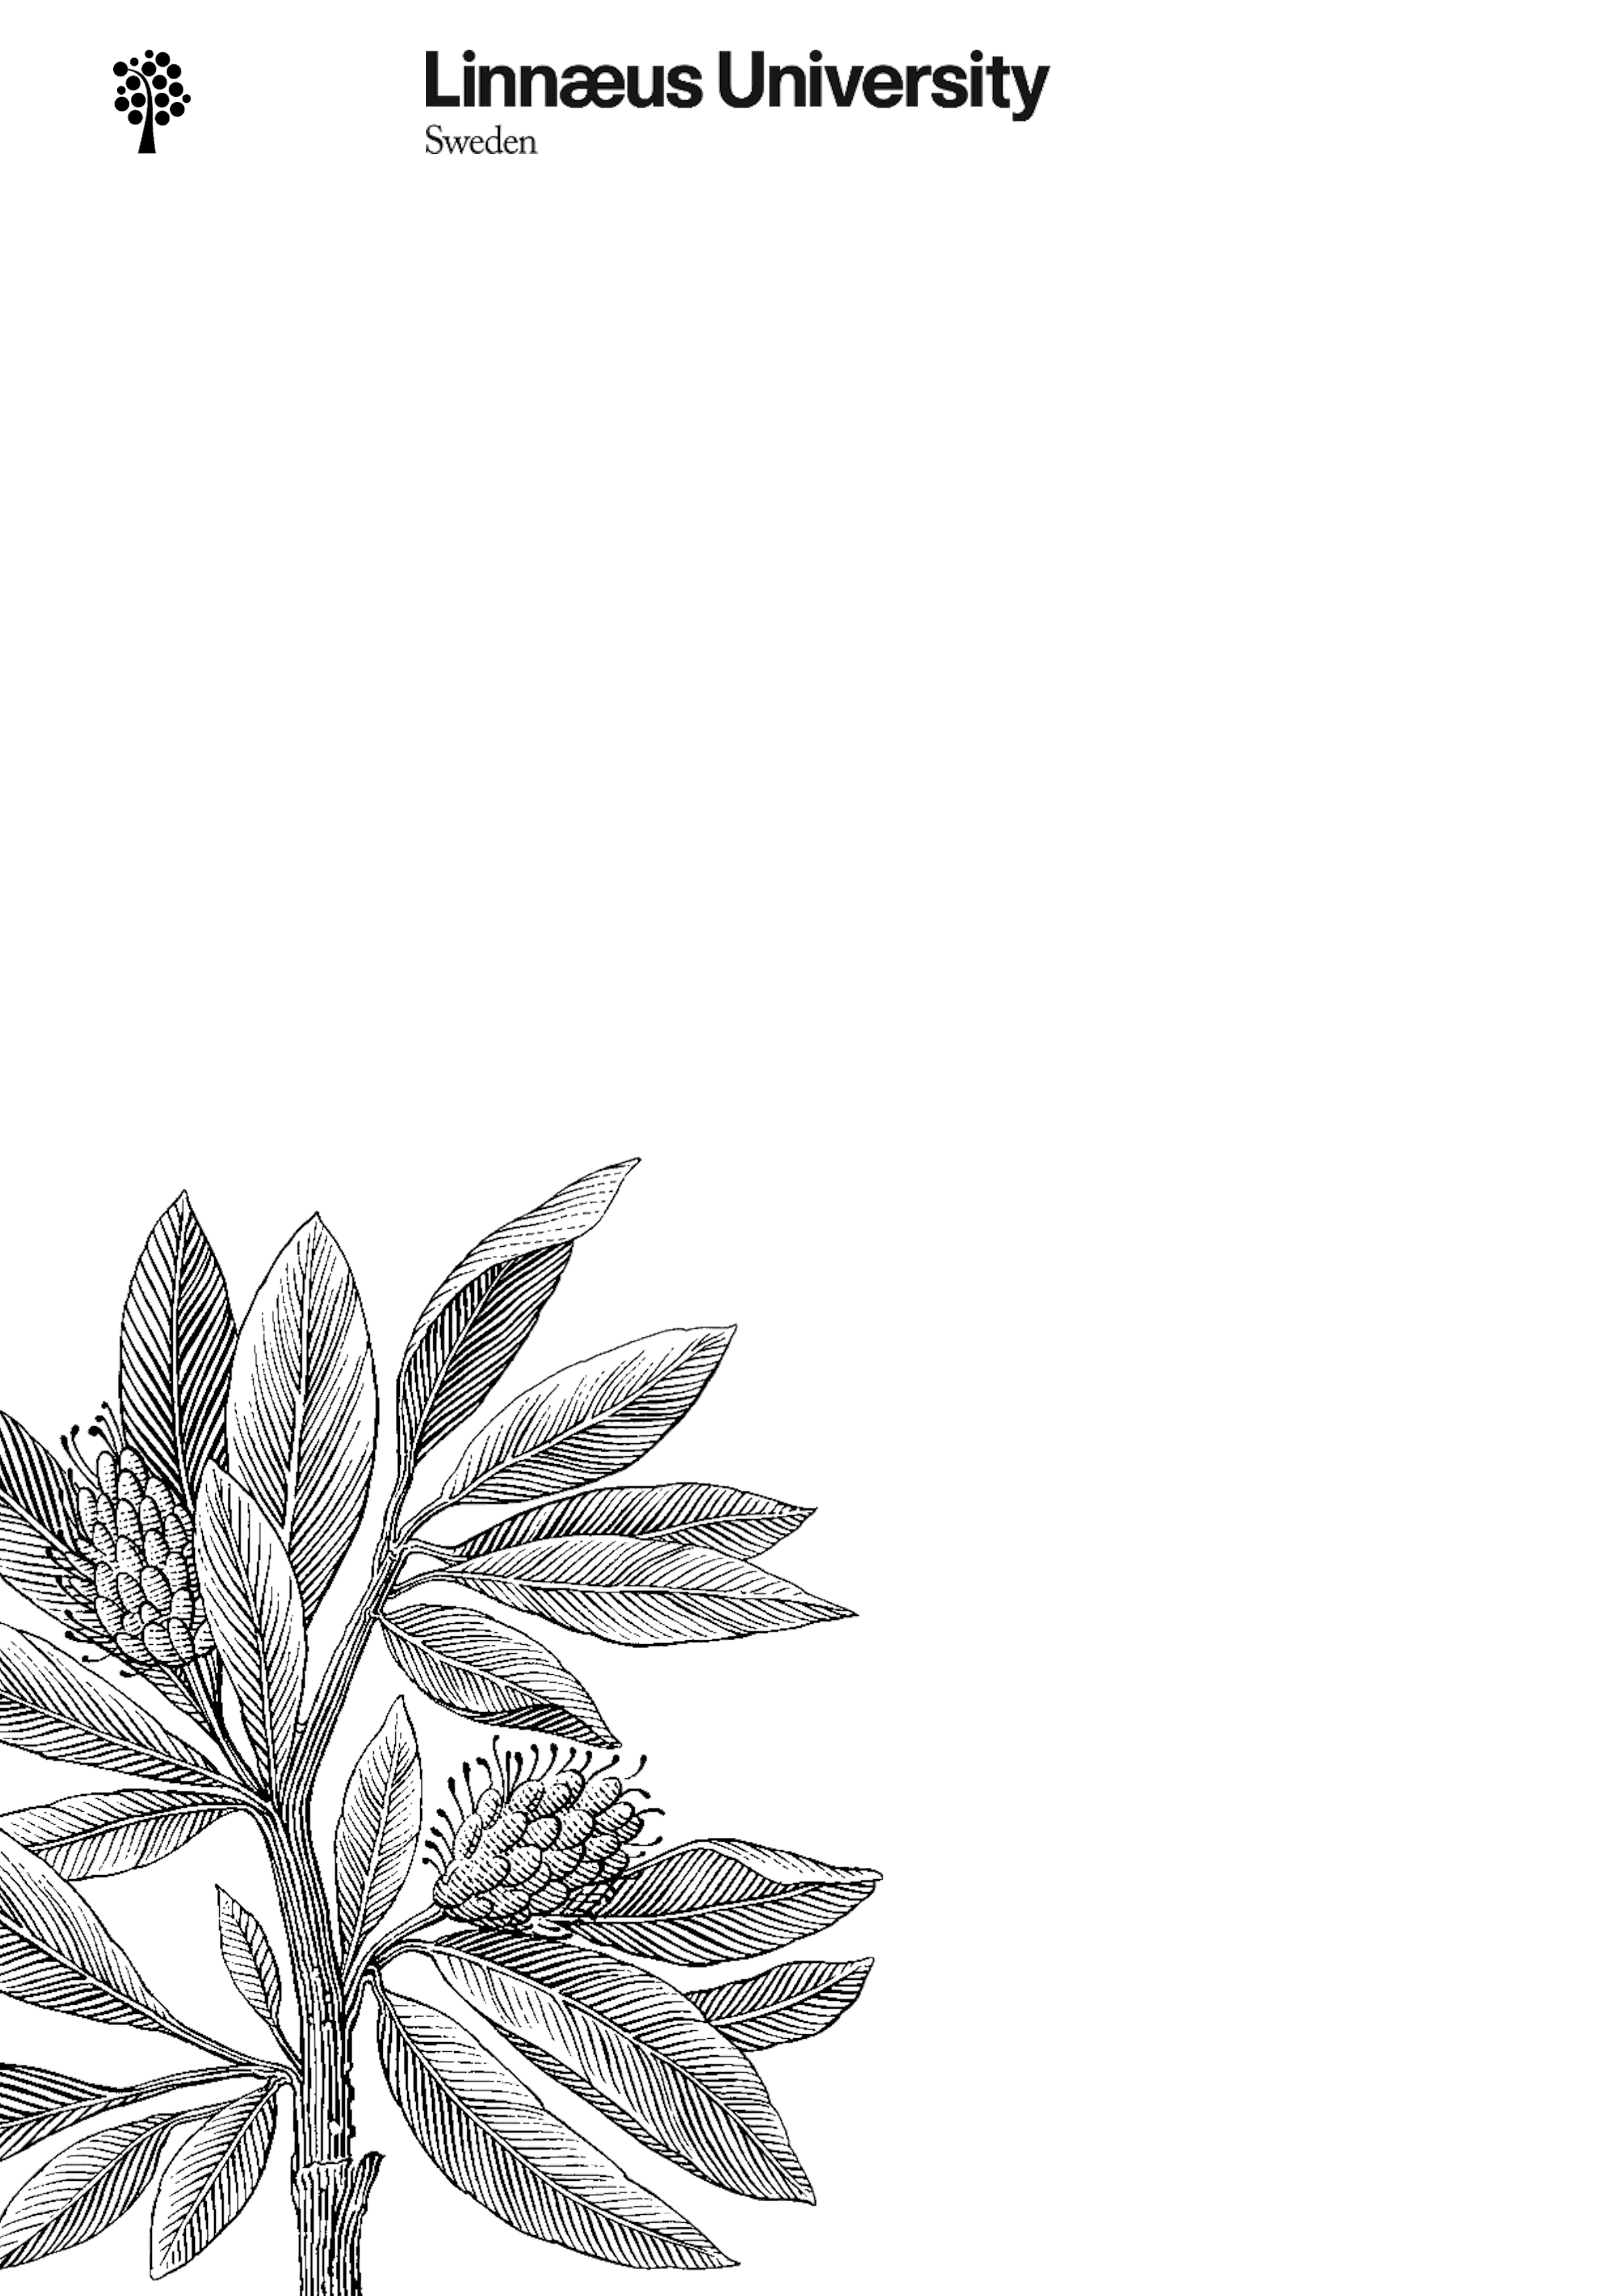
\includegraphics{titlepage_background}}
}
\usepackage{xcolor}

\usepackage{geometry}

\graphicspath{{logo/},{figures/}} % Set the default folder for images
%----------------------------------------------------------------------------------------
%	THEOREM STYLES
%---------------------------------------------------------------------------------------

\theoremstyle{definition} % Define theorem styles here based on the definition style (used for definitions and examples)
\newtheorem{definition}{Definition}

\theoremstyle{plain} % Define theorem styles here based on the plain style (used for theorems, lemmas, propositions)
\newtheorem{theorem}{Theorem}

\theoremstyle{remark} % Define theorem styles here based on the remark style (used for remarks and notes)

%----------------------------------------------------------------------------------------
%	HYPERLINKS
%---------------------------------------------------------------------------------------

\hypersetup{
%draft, % Uncomment to remove all links (useful for printing in black and white)
colorlinks=true, breaklinks=true, bookmarks=true,bookmarksnumbered,
urlcolor=webbrown, linkcolor=RoyalBlue, citecolor=webgreen, % Link colors
pdftitle={}, % PDF title
pdfauthor={\textcopyright}, % PDF Author
pdfsubject={}, % PDF Subject
pdfkeywords={}, % PDF Keywords
pdfcreator={pdfLaTeX}, % PDF Creator
pdfproducer={LaTeX with hyperref and ClassicThesis} % PDF producer
}



\newcommand*{\reporttitle}[1]{\def\rtitle{\normalfont\spacedallcaps #1}}
\newcommand*{\reportsubtitle}[1]{\def\rsubtitle{#1}}
\newcommand*{\documenttype}[1]{\def\doctype{#1}}
\newcommand*{\professor}[1]{\def\profname{#1}}
\newcommand*{\authors}[1]{\def\authorsname{\normalfont\spacedallcaps #1}}
\newcommand*{\email}[1]{\def\authorsemail{#1}}
\newcommand*{\authorssecond}[1]{\def\authorssecondname{\normalfont\spacedallcaps #1}}
\newcommand*{\emailsecond}[1]{\def\authorssecondemail{#1}}
\newcommand*{\coursename}[1]{\def\course{#1}}
\newcommand*{\coursecode}[1]{\def\coursecod{\texttt{#1}}}
\newcommand*{\semester}[1]{\def\sem{\texttt{#1}}} % Include the structure.tex file which specified the document structure and layout

\hyphenation{Fortran hy-phen-ation} % Specify custom hyphenation points in words with dashes where you would like hyphenation to occur, or alternatively, don't put any dashes in a word to stop hyphenation altogether



%----------------------------------------------------------------------------------------
%	DOCUMENT VARIABLES
%	Fill in the lines below to update the thesis template
%	If you wish to cite each of the variables defined below, look at the
%	section above for the citation command e.g. \examiner{} below is
%	defined as \examname above so you cite it as \examname
%----------------------------------------------------------------------------------------

\documenttype{Technical Report} %The document type
%-------------------------------------------------  
\reporttitle{Title of the report} % Your reoprt title - this is used in the title
%-------------------------------------------------  
\reportsubtitle{Subtitle of your report} %Subtitle of the report - this is used in the titlepage
%------------------------------------------------- 
\professor{Fredrik \textsc{Ahlgren}} % You supervisor's name (professor that holds the course)- this is used in the title page
%-------------------------------------------------   
\coursename{Project with Embedded System} %The course name
%------------------------------------------------- 
\coursecode{2DT304} %The course code
%------------------------------------------------- 
\semester{VT23} %The semester code of the course
%------------------------------------------------- 


\authors{Olof \textsc{Enström}} % Your name and surname- this is used in the title page and abstract
\email{oe222fh@student.lnu.se} %the author's email
%-------------------------------------------------

% Uncomment the following two lines if there is the second author also
% If there is a second authour, uncomment also the respective lines in the tile page
\authorssecond{Christoffer \textsc{Eid}} % name and surname of the second author- this is used in the title page and abstract
\emailsecond{ce223af@student.lnu.se} %the second author's email
%-------------------------------------------------

\date{} % An optional date to appear under the author(s)



%----------------------------------------------------------------------------------------

\begin{document}

%----------------------------------------------------------------------------------------
%	TITLE PAGE
%----------------------------------------------------------------------------------------
%\maketitle % Print the title/author/date block

% The new custom title page
\begin{titlepage} % Suppresses displaying the page number on the title page and the subsequent page counts as page 1
	
	\newgeometry{top=6mm, bottom=15mm, left=50mm, right=10mm}
	
	\BgThispage
	\raggedright
	\hspace*{-0.03\textwidth} % Whitespace between the vertical line and title page text
	\rule{0.5pt}{4cm} % Vertical line
	\hspace{0.005\textwidth} % Whitespace between the vertical line and title page text
	\fboxsep0pt
	\parbox[b]{0.85\textwidth}{ % Paragraph box for holding the title page text, adjust the width to move the title page left or right on the page
		{\huge \doctype}% Subtitle or further description
	}
	
	\vspace{4cm}
	
	\begin{minipage}{0.85\textwidth}
		{\Huge\bfseries \rtitle}\\[2\baselineskip] % Title
		{\LARGE\textit{\rsubtitle}}% Subtitle or further description
	\end{minipage}
	
	\vfill
	
	\raggedleft
	\begin{flushright}
		\vline
		\hspace{0.005\textwidth} % Whitespace between the vertical line and title page text
		\parbox[b]{0.45\textwidth}{ % Paragraph box for holding the title page text, adjust the width to move the title page left or right on the page
		
			{Author: \hfill\raggedleft\authorsname}\\ % Author name, lower case for consistent small caps
			{email: \hfill \authorsemail}\\
			%
			% Uncomment these two following two lines if there is a second author
			%
			{Author: \hfill\raggedleft\authorssecondname}\\ % Author name, lower case for consistent small caps
			{email: \hfill \authorssecondemail}\\
			\vfill
			{Professor: \hfill \profname}\\
			{Course: \hfill \coursecod}\\ % Author name, lower case for consistent small caps
			{Semester: \hfill \sem}\\	
	 	}
	\end{flushright}
	
	\restoregeometry
\end{titlepage}




%----------------------------------------------------------------------------------------
%	HEADERS
%----------------------------------------------------------------------------------------

\renewcommand{\sectionmark}[1]{\markright{\spacedlowsmallcaps{#1}}} % The header for all pages (oneside) or for even pages (twoside)
%\renewcommand{\subsectionmark}[1]{\markright{\thesubsection~#1}} % Uncomment when using the twoside option - this modifies the header on odd pages
\lehead{\mbox{\llap{\small\thepage\kern1em\color{halfgray} \vline}\color{halfgray}\hspace{0.5em}\rightmark\hfil}} % The header style

\pagestyle{scrheadings} % Enable the headers specified in this block


%----------------------------------------------------------------------------------------
%	TABLE OF CONTENTS & LISTS OF FIGURES AND TABLES
%----------------------------------------------------------------------------------------
\setcounter{tocdepth}{2} % Set the depth of the table of contents to show sections and subsections only

\tableofcontents % Print the table of contents

\clearpage

%Comment these lines if you don't want the lists of figures and/or tables
\listoffigures % Print the list of figures
\listoftables % Print the list of tables
\clearpage
%----------------------------------------------------------------------------------------
%	ABSTRACT
%----------------------------------------------------------------------------------------

%\section*{Abstract} % This section will not appear in the table of contents due to the star (\section*)

%\lipsum[1] % Dummy text

%----------------------------------------------------------------------------------------

%\newpage % Start the article content on the second page, remove this if you have a longer abstract that goes onto the second page


%----------------------------------------------------------------------------------------
%	MAIN CONTENT OF YOUR WORK
%----------------------------------------------------------------------------------------
%
% The command \input{filename} adds the content of the file "filename" in line
% The command \include{filename} does a \clearpage before adding the content of the file "filename"
%

%----------------------------------------------------------------------------------------
%	INTRODUCTION
%----------------------------------------------------------------------------------------
\section{Introduction}
\label{sec:introduction}

A statement requiring citation \cite{Figueredo:2009dg}. A statement requiring the reference to different document parts:
\begin{itemize}
	\item ... Section \ref{sec:introduction}
	\item ... see Section \ref{sec:results}
	\item ... please refer to Section \ref{sec:math}.
	\item Examples of wrong citation and reference : [??] and Section ??
	\item If citation or reference are done on wrong labels, the commands will return a double question mark ??
\end{itemize}

\lipsum[1-2] % Dummy text

Some mathematics in the text: $\cos\pi=-1$ and $\alpha$ \cite{Figueredo:2009dg}.
%----------------------------------------------------------------------------------------
%	METHODS
%----------------------------------------------------------------------------------------
\section{Methods}
\label{sec:methods}

\lipsum[5] % Dummy text

\begin{enumerate}[noitemsep] % [noitemsep] removes whitespace between the items for a compact look
\item First item in a list
\item Second item in a list
\item Third item in a list
\end{enumerate}

%------------------------------------------------

\subsection{Paragraphs}

\lipsum[6] % Dummy text

\paragraph{Paragraph Description} \lipsum[7] % Dummy text

\paragraph{Different Paragraph Description} \lipsum[8] % Dummy text

%------------------------------------------------

\subsection{Math}
\label{sec:math}
\lipsum[4] % Dummy text

\begin{equation}
\cos^3 \theta =\frac{1}{4}\cos\theta+\frac{3}{4}\cos 3\theta
\label{eq:refname2}
\end{equation}

\lipsum[5] % Dummy text

\begin{definition}[Gauss] 
To a mathematician it is obvious that
$\int_{-\infty}^{+\infty}
e^{-x^2}\,dx=\sqrt{\pi}$. 
\end{definition} 

\begin{theorem}[Pythagoras]
The square of the hypotenuse (the side opposite the right angle) is equal to the sum of the squares of the other two sides.
\end{theorem}

\begin{proof} 
We have that $\log(1)^2 = 2\log(1)$.
But we also have that $\log(-1)^2=\log(1)=0$.
Then $2\log(-1)=0$, from which the proof.
\end{proof}
%----------------------------------------------------------------------------------------
% Results
%----------------------------------------------------------------------------------------
\section{Results}\label{sec:results}

\subsection{WiFi Provisioning through Bluetooth}

The WiFi provisioning through Bluetooth system was successfully developed and implemented on the ESP32 microcontroller. The system enables efficient configuration of WiFi credentials on ESP32 devices through the use of a BLE-enabled device. The system was tested, and it was found to be reliable and effective in provisioning WiFi credentials without the need for code modification. The system was integrated as a component using the ESP-IDF framework, enabling easy integration by other developers. The use of BLE-enabled devices enhances security, making it a potential solution in the realm of IoT.

\subsection{OTA Updates}

The OTA update system was successfully developed and implemented on the ESP32 microcontroller. The system allows for remote firmware updates of the ESP32 board via a Wi-Fi connection, eliminating the need for a physical connection. The system was tested, and it was found to be reliable and effective in updating the firmware image without interrupting any critical tasks that the unit may be currently running. The \texttt{energy\_gateway\_ota} component was utilized to handle the initialization, download, verification, and activation of new firmware images. The component also integrates git tags as a versioning system, resulting in the update being aborted if the tags differ. The system also enables the possibility for rollback to a previous firmware image in the event of a failed update. However, this rollback functionality was not implemented in our project.

\subsection{UART Communication}

The implementation of serial communication on the ESP32 microcontroller was successful. The microcontroller was connected to a Heltec Wireless Stick~\ref{fig:serial_connection} and able to establish a serial communication channel with the Stick, running MicroPython, to receive and transmit data. The Wireless Stick was programmed to send random integers between 0 and 255 over serial at an interval. The ESP32 used the \texttt{uart\_read\_bytes()} function call, to read the bytes, with a timeout of 20 milliseconds, and place them in the \texttt{uartData} buffer (see figure \ref{fig:uart_read_bytes_function}). When a value greater than 250 or less than 5 was received, the microcontroller send back a value of 1 or 0, respectively, to the Wireless Stick. After every transmission, the buffer was cleared and the task yielded for 10 milliseconds, using \texttt{vTaskDelay(10 / portTICK\_PERIOD\_MS);} to not starve other tasks of resources.

The sending interval was tested at different frequencies, with promising results. When no other tasks were running, the device managed to catch all values sent at a data rate of 33Hz. Enabling the OTA task and running it every five seconds, the device was able to catch all values sent when the data rate was reduced to 20Hz.

\subsection{Concurrency}

First task thats creates is the UART task, which is given a priority of 19. This task is responsible for receiving data from the Wireless Stick and sending data back to the Wireless Stick. The task is given a priority of 19 to ensure that it is not preempted by any other tasks. The task is then put into a while loop, where it waits for data to be received. When data is received, the task checks if the data is greater than 250 or less than 5. If the data is greater than 250, the task sends a value of 1 back to the Wireless Stick. If the data is less than 5, the task sends a value of 0 back to the Wireless Stick. The task then yields for 10 milliseconds, using \texttt{vTaskDelay(10 / portTICK\_PERIOD\_MS);}.

After the UART task is created, the OTA task is created. This task is given a priority of 2. This task is responsible for checking for new firmware images and updating the firmware image if a new one is available. The task is given a priority of 2 to ensure that it does not preemp any other tasks. After the task has been run once its removed from the task list, a timer is started that will run the task again after 24 hours. When the timer expires, the task is once again placed in the task list, on a low priority of 2.


%clear the remaining space of the page and pushes the following content to the new page
\clearpage


%----------------------------------------------------------------------------------------
%	BIBLIOGRAPHY
%----------------------------------------------------------------------------------------
\renewcommand{\refname}{\spacedlowsmallcaps{References}} % For modifying the bibliography heading

\bibliographystyle{unsrt}

\bibliography{bibliography.bib} % The file containing the bibliography

%----------------------------------------------------------------------------------------

\end{document}